% =============================================================================
% artigo-alpha: versão preliminar do artigo (22/10/2026), só com as três testnets públicas.
%
% - Serve de base para a escrita final; o texto definitivo vai para o template do
%   COTB 2027 (paper/template_cotb2027.tex), sem mudar a formatação do template.
% - Todos os números vêm de pesquisa/3-resultados/resultados.md (npm run analisar).
%   Se a análise for refeita, atualize as tabelas daqui junto.
% - \pendente{...} marca o que falta escrever, conferir ou citar. Nenhum pode
%   sobrar na versão enviada.
% - Regras do template (matriz, seção 13): até 6 páginas com referências; título,
%   abstract e keywords em inglês; citações numéricas; versão de avaliação anônima;
%   Declaração de Uso de IA obrigatória; não identificar o banco parceiro.
%
% Compilar (dentro de artigo/): latexmk -pdf artigo-alpha.tex   (TinyTeX em ~/.TinyTeX; binários em ~/.local/bin)
% Pacote faltando: tlmgr install <pacote>
% =============================================================================
\documentclass[10pt,a4paper]{article}

\usepackage[T1]{fontenc}
\usepackage[utf8]{inputenc}
\usepackage[english,brazilian]{babel}
\usepackage{lmodern}
\usepackage[margin=2.2cm]{geometry}
\usepackage{graphicx}
\usepackage{booktabs}
\usepackage{tabularx}
\usepackage{multirow}
\usepackage{amsmath}
\usepackage{xcolor}
\usepackage{caption}
\usepackage[hidelinks]{hyperref}

\graphicspath{{../pesquisa/3-resultados/graficos/}{figuras/}}

\newcommand{\pendente}[1]{\textcolor{red}{[#1]}}
\newcommand{\fn}[1]{\texttt{#1}}

\title{Seleção de rede blockchain para crédito interfinanceiro overnight com liquidação DvP: uma avaliação multicritério em testnets públicas\\[0.6em]
\large Blockchain network selection for overnight interbank lending with DvP settlement: a multi-criteria evaluation on public testnets}
\author{\pendente{Autores omitidos na versão de avaliação}}
\date{}

\begin{document}
\maketitle

% -----------------------------------------------------------------------------
\begin{otherlanguage}{english}
\begin{abstract}
Overnight interbank lending still relies on manual limit checks and reconciliation, which delay settlement and increase counterparty risk. This paper asks which blockchain network is most suitable for running an overnight interbank lending protocol with delivery-versus-payment (DvP) settlement. We frame the choice as a multi-attribute decision problem with five criteria weighted by the Analytic Hierarchy Process (AHP): resilience under load (29.78\%), contract security (29.78\%), latency (15.78\%), cost (15.78\%) and EVM compatibility (8.88\%), aggregated by a weighted sum over min-max normalized scores. Three public networks were evaluated by deploying the same unmodified Solidity contract on their public testnets (Ethereum Sepolia, Avalanche Fuji and Monad) and executing 1,095 transactions in a single collection window: 30 sequential lending cycles plus 10 cancellations, and 255 acceptances in concurrent batches of 10, 25 and 50. No transaction failed. Monad ranked first (90.1 of 100), with a median inclusion latency of 0.99~s and a cycle cost of US\$~0.0014 at mainnet prices, followed by Avalanche (86.0; 2.64~s; US\$~0.029) and Ethereum (58.5; 11.04~s; US\$~0.296). The ranking held in all 17 weight scenarios, because resilience, security and compatibility did not discriminate between the three EVM networks. We also report that a protocol upgrade activated on Sepolia during the study made the lending cycle consume 3.50 times the gas measured under the rules still in force on Ethereum mainnet, which breaks the usual assumption that testnet gas equals mainnet gas. \pendente{revisar; até cerca de 250 palavras}
\end{abstract}

\noindent\textbf{Keywords:} blockchain selection; multi-criteria decision making; AHP; delivery versus payment; interbank lending; benchmark.
\end{otherlanguage}

\vspace{0.5em}
\noindent\textbf{Palavras-chave:} seleção de blockchain; decisão multicritério; AHP; entrega contra pagamento; crédito interfinanceiro; benchmark.

% -----------------------------------------------------------------------------
\section{Introdução}

A gestão de liquidez interbancária de curtíssimo prazo ainda depende de checagens manuais de limite e de conciliação entre as partes. Esse processo cria um intervalo entre a negociação e a liquidação, o que aumenta o risco de contraparte e a complexidade do fechamento diário de caixa. Um protocolo em blockchain pode automatizar a oferta, a checagem de limite e a liquidação na mesma transação, com entrega contra pagamento (DvP) \cite{bis1992dvp,cpss2012pfmi}.

A escolha da rede que executaria esse protocolo, porém, costuma ser feita por preferência técnica. Estudos de seleção de plataformas blockchain mostram que a escolha depende de critérios que entram em conflito, como desempenho, custo e segurança, e que um método de decisão explícito torna a escolha auditável \cite{farshidi2020,baninemeh2023,six2020}.

Este trabalho responde à seguinte questão de pesquisa: \emph{qual rede blockchain é mais adequada para executar um protocolo de concessão de crédito interfinanceiro overnight com liquidação por entrega contra pagamento (DvP)?} O protocolo avaliado foi desenvolvido numa parceria acadêmica com uma instituição financeira e usa ativos simulados, sem integração com sistemas de produção.

As contribuições são: (i) um modelo de decisão multicritério com cinco critérios e pesos pelo AHP, aplicado a um caso financeiro concreto; (ii) medições do mesmo contrato, sem alteração, nas testnets públicas de três redes compatíveis com a EVM, coletadas na mesma janela; e (iii) a evidência de que uma atualização de protocolo na Sepolia, ativada durante o estudo, invalida a premissa de que o gas medido na testnet representa o da mainnet. \pendente{ajustar as contribuições ao texto final}

O restante do artigo está organizado assim: a Seção~\ref{sec:fundamentacao} apresenta os conceitos e os trabalhos relacionados; a Seção~\ref{sec:metodo}, o método e o modelo de decisão; a Seção~\ref{sec:resultados}, os resultados; a Seção~\ref{sec:discussao}, a discussão e as ameaças à validade; e a Seção~\ref{sec:conclusao}, as conclusões.

% -----------------------------------------------------------------------------
\section{Fundamentação Teórica}\label{sec:fundamentacao}

\paragraph{DvP e liquidação atômica.} Na entrega contra pagamento, o ativo só é entregue se o pagamento acontecer. Sem esse vínculo existe o risco de principal: perder o valor inteiro da operação porque uma parte entregou e a outra não \cite{bis1992dvp}. O Princípio~12 dos PFMI exige que a liquidação de uma obrigação dependa da liquidação da outra \cite{cpss2012pfmi}. Em blockchain, isso se obtém com liquidação atômica: um contrato liga as duas transferências, e uma só ocorre se a outra também ocorrer \cite{bis2020qr}.

\paragraph{Decisão multicritério.} A escolha entre uma lista fechada de alternativas, avaliadas em critérios que podem entrar em conflito, é um problema de decisão multiatributo (MADM). O AHP deriva os pesos de comparações par a par entre critérios e verifica a consistência dos julgamentos \cite{saaty2001}. A soma ponderada (WSM) agrega as notas normalizadas \pendente{referência revisada por pares para o WSM}. Como a normalização depende do conjunto de alternativas, incluir ou retirar uma alternativa pode inverter a ordem das demais \cite{belton1983}; por isso a lista é fechada antes do cálculo. A análise de sensibilidade testa se a ordem se mantém quando os pesos mudam \cite{triantaphyllou1997}.

\subsection{Trabalhos Relacionados}

Farshidi et al.\ propõem um modelo de decisão para seleção de plataformas blockchain e o aplicam em três estudos de caso industriais \cite{farshidi2020}; Baninemeh et al.\ usam a mesma abordagem para plataformas de DAO e tratam requisitos obrigatórios como filtro, e não como critério \cite{baninemeh2023}. Six et al.\ combinam dados declarados e medidos para escolher uma blockchain \cite{six2020}. Do lado das medições, o Diablo compara blockchains sob cargas realistas e mostra que números declarados pelas redes costumam não ser reproduzíveis \cite{gramoli2023}; Lazăr et al.\ comparam o custo de implantação e execução de contratos entre redes EVM \cite{lazar2025}; e Javed et al.\ medem a latência de contratos na Ethereum sob envios simultâneos \cite{javed2025}. \pendente{posicionar este trabalho: caso financeiro com DvP, mesmo contrato sem alteração, coleta simultânea nas três testnets}

% -----------------------------------------------------------------------------
\section{Método}\label{sec:metodo}

\subsection{Definição do Problema e Método}

O problema é tratado como MADM com três alternativas e cinco critérios. Os pesos vêm do AHP; as notas são normalizadas por min-max (Eq.~\ref{eq:minmax}) e agregadas por soma ponderada (Eq.~\ref{eq:wsm}). Em caso de empate (máximo igual ao mínimo), todas as redes recebem nota~1, porque nenhuma deve ser penalizada num critério em que todas são iguais.
\begin{equation}\label{eq:minmax}
r_{ij} = \frac{x_{ij} - \min_i x_{ij}}{\max_i x_{ij} - \min_i x_{ij}} \;\text{(benefício)}, \qquad
r_{ij} = \frac{\max_i x_{ij} - x_{ij}}{\max_i x_{ij} - \min_i x_{ij}} \;\text{(custo)}
\end{equation}
\begin{equation}\label{eq:wsm}
P(A_i) = \sum_{j=1}^{5} w_j \, r_{ij}
\end{equation}

A sensibilidade é avaliada em 16 cenários além do base: pesos iguais (S1); cada peso aumentado e reduzido em 50\%, um de cada vez, com renormalização (S2, 10 cenários); e cada critério retirado, um de cada vez (S3, 5 cenários).

\subsection{Modelo de Decisão}

\paragraph{Alternativas e por que foram escolhidas.} A Tabela~\ref{tab:redes} lista as redes avaliadas. Cada uma precisou atender a três condições. A primeira é executar transações de forma atômica, condição para a liquidação DvP (ver condição de elegibilidade, adiante). A segunda é executar o contrato do protocolo, escrito em Solidity e testado com Foundry, sem reescrita: assim a comparação mede a rede, e não uma nova implementação do contrato. A terceira é ter testnet pública de acesso livre, com faucet, para que as três fossem medidas nas mesmas condições (tráfego de terceiros e RPC público) e na mesma janela.

Dentro dessas condições, as três redes cobrem perfis diferentes de rede EVM pública. A Ethereum é a rede de origem da EVM e o ambiente em que o protocolo já está implantado (Sepolia); serve de referência para as demais \cite{ethereum2024gasper}. A Avalanche (C-Chain) executa o mesmo bytecode com consenso Snowman e finalidade declarada inferior a 1~s \cite{avalanche2024consensus}. A Monad é uma rede EVM voltada a desempenho, com execução paralela e finalidade declarada de 600~ms \cite{monad2024bft}; como esses números são divulgados pelo próprio projeto, a medição serve também para verificá-los \cite{gramoli2023}. Na etapa exploratória, Solana e Stellar (contratos em Rust, executados em SBF e WebAssembly) e Miden (Rust e Miden Assembly, ainda sem mainnet) foram descartadas por exigirem a reescrita do contrato.

\begin{table}[ht]
\centering
\caption{Redes avaliadas.}\label{tab:redes}
\small
\begin{tabularx}{\linewidth}{@{}lllX@{}}
\toprule
Rede & Testnet (chain ID) & Consenso & Finalidade declarada \\
\midrule
Ethereum & Sepolia (11155111) & PoS (Gasper), slots de 12~s & Não imediata: 2 épocas, cerca de 12,8~min \cite{ethereum2024gasper} \\
Avalanche (C-Chain) & Fuji (43113) & Snowman & Menos de 1~s \cite{avalanche2024consensus} \\
Monad & Monad Testnet (10143) & MonadBFT, bloco mínimo de 300~ms & 2 slots, 600~ms \cite{monad2024bft} \\
\bottomrule
\end{tabularx}
\end{table}

\paragraph{Condição de elegibilidade.} A liquidação atômica não é critério, e sim condição para entrar na lista: as três redes executam transações de forma atômica, e um critério com a mesma nota em todas as alternativas não altera a ordem \cite{baninemeh2023}. No protocolo, o aceite da oferta consome o limite do tomador, transfere o real tokenizado (ERC-20) do ofertante para o tomador e emite para o ofertante o NFT de posição (ERC-721), tudo na mesma transação. \pendente{citar a documentação de atomicidade de cada rede}

\paragraph{Critérios e pesos.} A Tabela~\ref{tab:criterios} resume os critérios. Os pesos são o autovetor principal da matriz de comparações da Tabela~\ref{tab:ahp}, obtida por uma regra de níveis (alto: C1 e C2; médio: C3 e C4; baixo: C5). A razão de consistência é CR~$=0{,}0030$ ($\lambda_{\max}=5{,}0133$; CI~$=0{,}0033$; RI~$=1{,}12$), abaixo do limite de 0,10 \cite{saaty2001}. \pendente{fonte original do RI e do limite}

\begin{table}[ht]
\centering
\caption{Critérios, pesos e origem dos dados.}\label{tab:criterios}
\small
\begin{tabularx}{\linewidth}{@{}lrlX@{}}
\toprule
Critério & Peso & Sentido & Valor que entra na matriz \\
\midrule
C1 Resiliência & 29,78\% & benefício & Taxa de sucesso agregada no teste de carga (T2), medida \\
C2 Segurança do contrato & 29,78\% & benefício & Média de M1 verificação formal (declarado), M2 complexidade ciclomática do código (medido) e M3 confidencialidade (declarado) \\
C3 Latência & 15,78\% & custo & Mediana da latência do aceite no T1, do envio até o recibo, medida \\
C4 Custo & 15,78\% & custo & M1 custo médio do ciclo em USD a preços da mainnet (medido); M2 infraestrutura (declarado; descritivo, fora da pontuação) \\
C5 Compatibilidade EVM & 8,88\% & benefício & Sem alteração (1,0), compilador modificado (0,5) ou reescrita (0,0), confirmado na implantação \\
\bottomrule
\end{tabularx}
\end{table}

\begin{table}[ht]
\centering
\caption{Matriz de comparações par a par do AHP.}\label{tab:ahp}
\small
\begin{tabular}{@{}lccccc@{}}
\toprule
 & C1 & C2 & C3 & C4 & C5 \\
\midrule
C1 & 1 & 1 & 2 & 2 & 3 \\
C2 & 1 & 1 & 2 & 2 & 3 \\
C3 & 1/2 & 1/2 & 1 & 1 & 2 \\
C4 & 1/2 & 1/2 & 1 & 1 & 2 \\
C5 & 1/3 & 1/3 & 1/2 & 1/2 & 1 \\
\bottomrule
\end{tabular}
\end{table}

As medidas de C2 e C4 são combinadas por média simples. A complexidade ciclomática \cite{mccabe1976} conta só o código da equipe (sem bibliotecas), com $M = 49$ (24 funções e 25 pontos de decisão); como o código é o mesmo nas três redes, a medida empata. Para C2-M1, o SMTChecker integra o compilador Solidity \cite{solidity2024smt}, nota 1,0 nas três. Para C2-M3, as três redes são públicas e qualquer pessoa lê os eventos do contrato, nota 0. O custo de infraestrutura (C4-M2) foi levantado para três nós em nuvem (AWS \fn{us-east-1}, sob demanda, 19/10/2026): US\$~376,68 por mês na Ethereum, US\$~1.502,34 na Avalanche e US\$~8.681,38 na Monad, cuja documentação exige servidor físico (US\$~1.563,66 com instância virtual). Por decisão da equipe, esses valores são descritivos e C4 usa só C4-M1.

\subsection{Coleta de Dados}

\paragraph{Protocolo e ciclo medido.} O ciclo medido é \fn{approve} (autorização no valor exato) $+$ \fn{createOffer} $+$ \fn{acceptOffer} \cite{eip20}. Em cada rede foi feita uma implantação nova com a mesma configuração (Solidity 0.8.24, otimizador com 200 execuções), sem alteração de código.

\paragraph{Testes.} O T1 executa 30 ciclos em sequência e 10 cancelamentos (110 transações por rede); a mediana da latência do \fn{acceptOffer} entra em C3, e a média do custo do ciclo entra em C4-M1. O T2 dispara 255 aceites simultâneos, em lotes de 10, 25 e 50 com 3 rodadas, e a taxa de sucesso agregada entra em C1. A latência é medida do envio real (após a estimativa de gas) até o recibo. As falhas são classificadas pelo nome do erro em contrato (A), cliente (B), RPC (C) e rede (D); só a categoria D conta contra a rede \cite{hyperledger2018metrics,lazar2025}.

\paragraph{Custo.} Como tokens de testnet não têm valor, o custo é o gas medido na testnet multiplicado pela mediana do preço do gas na mainnet e pela cotação do token nativo, ambos amostrados durante a coleta \cite{ethereum2024gas}. A Monad cobra o \emph{gas limit} enviado, e não o gas usado \cite{monad2024gas}; o custo dela usa o limite (estimativa $\times$ 1,2, igual em todas as redes).

\paragraph{Ambiente.} As três testnets foram coletadas em paralelo em 16/10/2026, entre 22:40 e 23:22 UTC, a partir da mesma máquina e com RPC público gratuito. Os preços de referência são a mediana de 9 amostras na mesma janela (\fn{eth\_feeHistory} e CoinGecko): Ethereum 0,081~gwei a US\$~2.422,04; Avalanche 6,77~gwei a US\$~9,97; Monad 103~gwei a US\$~0,0229. Scripts e dados brutos estão disponíveis \pendente{link do repositório, anonimizado na versão de avaliação}.

% -----------------------------------------------------------------------------
\section{Resultados}\label{sec:resultados}

Foram medidas 1.095 transações (365 por rede), todas confirmadas: nenhuma falha de nenhuma categoria no T1 nem no T2. A Tabela~\ref{tab:medidas} resume as medidas e a Figura~\ref{fig:latencia} mostra a distribuição da latência no T1. As três redes incluíram todas as operações do T1 em menos dos 30~s exigidos pelo requisito de confirmação do protocolo.

\begin{table}[ht]
\centering
\caption{Medidas por rede (coleta de 16/10/2026).}\label{tab:medidas}
\small
\begin{tabularx}{\linewidth}{@{}lXXXXr@{}}
\toprule
Rede & T1: mediana (p95; máx.) & T2: sucesso & T2: mediana por lote (10; 25; 50) & Gas do ciclo & Custo do ciclo \\
\midrule
Monad & 0,99~s (1,56; 1,74) & 100\% (255/255) & 0,80; 1,04; 1,10~s & 602.935\textsuperscript{a} & US\$~0,0014 \\
Avalanche & 2,64~s (3,03; 3,13) & 100\% (255/255) & 2,47; 2,40; 3,49~s & 429.924 & US\$~0,0290 \\
Ethereum & 11,04~s (11,98; 22,02) & 100\% (255/255) & 9,39; 8,85; 7,65~s & 1.502.836 & US\$~0,2961 \\
\bottomrule
\multicolumn{6}{@{}l}{\footnotesize \textsuperscript{a} Gas limit, que é o que a Monad cobra; nas demais, gas usado.}
\end{tabularx}
\end{table}

\begin{figure}[ht]
\centering
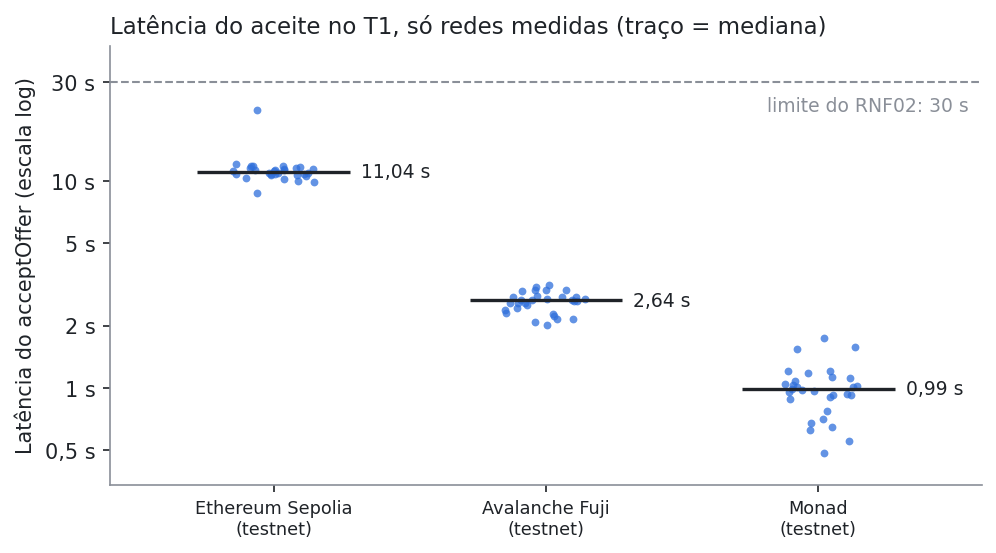
\includegraphics[width=0.85\linewidth]{latencia_t1.png}
\caption{Latência do \fn{acceptOffer} no T1 (30 aceites por rede, escala logarítmica). \pendente{refazer a figura em inglês ou sem título interno, conforme o template}}\label{fig:latencia}
\end{figure}

A Tabela~\ref{tab:notas} traz as notas normalizadas e a pontuação. A Monad ficou em primeiro lugar com 90,1 pontos, seguida pela Avalanche (86,0) e pela Ethereum (58,5). A Figura~\ref{fig:custo} compara o custo do ciclo.

\begin{table}[ht]
\centering
\caption{Notas normalizadas (0 a 1) e pontuação ponderada (0 a 100), cenário base.}\label{tab:notas}
\small
\begin{tabular}{@{}clcccccr@{}}
\toprule
Posição & Rede & C1 & C2 & C3 & C4 & C5 & Pontuação \\
\midrule
1 & Monad & 1,00 & 0,67 & 1,00 & 1,00 & 1,00 & \textbf{90,1} \\
2 & Avalanche & 1,00 & 0,67 & 0,84 & 0,91 & 1,00 & 86,0 \\
3 & Ethereum & 1,00 & 0,67 & 0,00 & 0,00 & 1,00 & 58,5 \\
\bottomrule
\end{tabular}
\end{table}

\begin{figure}[ht]
\centering
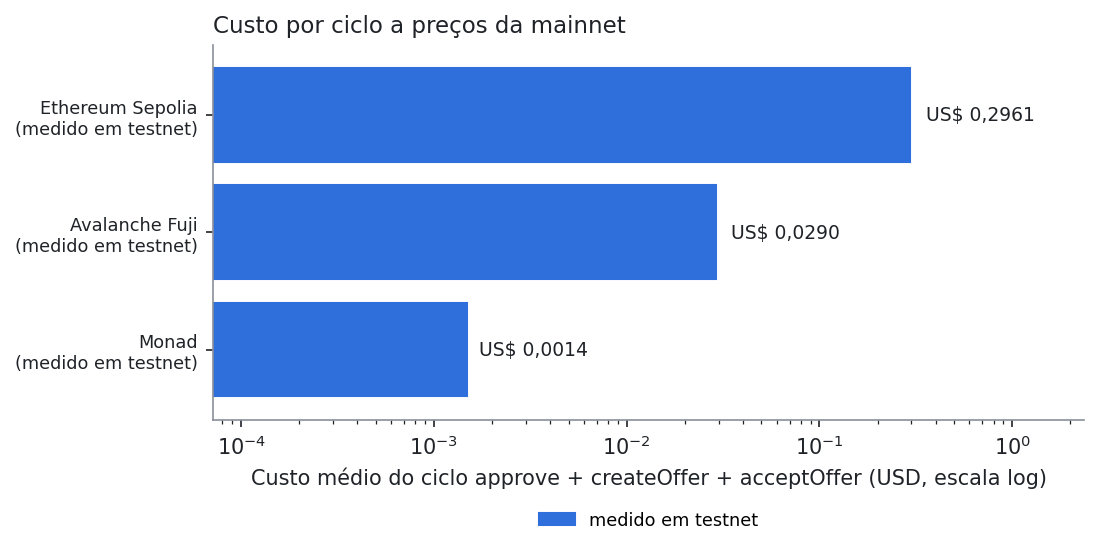
\includegraphics[width=0.85\linewidth]{custo_ciclo.png}
\caption{Custo médio do ciclo a preços da mainnet (escala logarítmica). \pendente{idem}}\label{fig:custo}
\end{figure}

\paragraph{Sensibilidade.} A ordem Monad, Avalanche e Ethereum se manteve nos 17 cenários (base, S1, S2 e S3). A menor pontuação da Monad foi 85,9 (S3 sem C1) e a maior, 100,0 (S3 sem C2); a diferença para a Avalanche variou de 1,8 (S3 sem C3) a 5,8 pontos (S3 sem C1 e S3 sem C2).

\paragraph{Custo de infraestrutura.} Com C4-M2 na pontuação, a ordem passaria a depender da instância da Monad: com servidor físico, Avalanche 85,7, Monad 82,2 e Ethereum 66,4; com instância virtual, Monad 82,2, Avalanche 79,2 e Ethereum 66,4. \pendente{discutir na Seção 5: a recomendação é sensível ao custo de operar um nó da Monad}

\paragraph{Gas da Sepolia após o Glamsterdam.} A Sepolia ativou em 06/10/2026 a atualização Glamsterdam, que encarece a criação de estado \cite{glamsterdam2026}; a mainnet da Ethereum ainda usa as regras anteriores. A Tabela~\ref{tab:glamsterdam} compara o gas do ciclo na Sepolia com o gas na Fuji, que executa o mesmo bytecode com as regras anteriores. O ciclo gastou 3,50 vezes mais na Sepolia. A matriz usa o gas da Sepolia, como define o método; com o gas da Fuji, o custo do ciclo da Ethereum cai de US\$~0,296 para US\$~0,085, a Ethereum continua a mais cara e a ordem não muda (a Avalanche passaria de 86,0 para 82,2 pontos).

\begin{table}[ht]
\centering
\caption{Gas por função: Sepolia (com Glamsterdam) e Fuji (regras anteriores).}\label{tab:glamsterdam}
\small
\begin{tabular}{@{}lrrr@{}}
\toprule
Função & Sepolia & Fuji & Razão \\
\midrule
\fn{approve} & 128.257 & 46.337 & 2,77$\times$ \\
\fn{createOffer} & 927.005 & 220.324 & 4,21$\times$ \\
\fn{acceptOffer} & 446.758 & 163.120 & 2,74$\times$ \\
\fn{cancelOffer} & 133.830 & 51.810 & 2,58$\times$ \\
\midrule
Ciclo completo & 1.502.836 & 429.924 & 3,50$\times$ \\
\bottomrule
\end{tabular}
\end{table}

% -----------------------------------------------------------------------------
\section{Discussão}\label{sec:discussao}

\subsection{Interpretação dos Resultados}

Com três redes EVM públicas executando o mesmo código, três dos cinco critérios não diferenciaram as alternativas: C1 empatou em 100\% de sucesso; C2 teve a mesma nota nas três (mesma linguagem, mesmo código, mesma visibilidade pública); e C5 foi 1,0 em todas, porque o contrato foi implantado sem alteração. O ranking foi decidido por latência e custo, que somam 31,56\% do peso. Como a Monad teve a melhor nota nesses dois critérios e a Ethereum a pior, a ordem se mantém para quaisquer pesos não negativos, o que explica a estabilidade da análise de sensibilidade. \pendente{discutir se o resultado responde à QP ou se, para este conjunto de redes, a decisão se reduz a latência e custo}

A latência de inclusão não conta toda a história. Na Ethereum, a operação só se torna definitiva cerca de 12,8~min após a inclusão \cite{ethereum2024gasper}, o que pesa num produto overnight com janela de liquidação curta; na Avalanche e na Monad a finalidade declarada é inferior a 1~s \cite{avalanche2024consensus,monad2024bft}. Nenhuma das três oferece confidencialidade entre participantes na própria rede: valores, taxas e contrapartes ficam visíveis a qualquer observador, e o sigilo exigido em operações interbancárias teria de ser tratado na aplicação. As três também têm conjunto aberto de validadores, sem governança institucional identificada. \pendente{relacionar com o requisito de sigilo}

O custo absoluto é baixo nas três redes (de US\$~0,0014 a US\$~0,30 por ciclo), mas a diferença relativa é de duas ordens de grandeza. Na Monad, o custo depende do gas limit enviado pelo cliente, e não só do trabalho executado.

Sob carga, a Avalanche apresentou 3 aceites de 64~s no lote de 50 da primeira rodada, acima do limite de 30~s. O horário coincide com uma pausa registrada do observador de blocos do coletor. \pendente{conferir se é efeito da medição antes de citar; a latência do T2 não entra na matriz}

\subsection{Ameaças à Validade e Limitações}\label{sec:ameacas}

\begin{itemize}
\item \textbf{Testnet não é mainnet.} O tráfego é menor, e o custo supõe que o gas da testnet é igual ao da mainnet; para a Ethereum essa premissa deixou de valer durante o estudo (Glamsterdam).
\item \textbf{Uma única janela de coleta.} As três testnets foram coletadas em paralelo, numa janela de 42~min, da mesma máquina e com RPC público; a variação do tráfego ao longo do tempo não foi observada.
\item \textbf{Carga limitada.} Com até 50 aceites simultâneos nenhuma rede falhou; C1 não separou as redes e não mede a capacidade máxima.
\item \textbf{Critérios que empataram.} C1, C2 e C5 deram a mesma nota às três redes; a estrutura de cinco critérios foi pensada para uma lista mais variada.
\item \textbf{Conjunto de redes.} As três redes são públicas, então a confidencialidade não diferenciou as alternativas e a conclusão vale para redes públicas. Incluir ou retirar uma rede muda as notas min-max das demais \cite{belton1983}; por isso a lista foi fechada antes do cálculo.
\item \textbf{Pesos e escalas.} Os julgamentos do AHP vieram de uma regra por níveis, e não de comparações independentes; as escalas qualitativas (C2-M1, C2-M3, C5) foram definidas pela equipe; as medidas internas de C2 e C4 usam média simples.
\item \textbf{Latência e finalidade.} A latência mede a inclusão no bloco; a janela do requisito de 30~s também inclui backend e interface, e inclusão não é finalidade.
\item \textbf{Dados declarados.} A finalidade e parte das escalas vêm da documentação das próprias redes, não verificada por terceiros \cite{gramoli2023}.
\item \textbf{Generalização.} Um único protocolo foi avaliado; os resultados valem para este caso de uso.
\end{itemize}
\pendente{condensar para caber nas 6 páginas}

% -----------------------------------------------------------------------------
\section{Conclusões e Trabalhos Futuros}\label{sec:conclusao}

Entre as três redes públicas avaliadas, a Monad é a mais adequada para o protocolo de crédito interfinanceiro overnight segundo o modelo de decisão: foi a mais rápida e a mais barata, executou o contrato sem alteração e liderou em todos os cenários de pesos. A Avalanche é uma alternativa próxima, e a Ethereum pública mostrou-se inadequada como camada de liquidação para este caso, pela latência, pelo tempo até a finalidade e pelo custo. O estudo também mostra que testnets podem mudar de regras durante uma coleta, o que exige registrar a versão do protocolo junto com as medições de custo.

Como trabalhos futuros: repetir o T2 com carga maior, até haver falhas; incluir o custo de infraestrutura na pontuação com mais de um provedor; e repetir a coleta em várias janelas. \pendente{revisar}

% -----------------------------------------------------------------------------
\section*{Agradecimentos}
\pendente{omitidos na versão de avaliação}

\section*{Declaração de Uso de IA}
\pendente{obrigatória nas duas versões: descrever quais ferramentas de IA foram usadas, em quais etapas (código de coleta e análise, revisão de texto etc.) e como a equipe verificou o resultado}

\bibliographystyle{unsrt} % trocar pelo estilo numérico ACM do template
\bibliography{referencias}

\end{document}
